\chapter{Soluzioni di viscosità}
In questa sezione richiamiamo alcune nozioni base sulle soluzioni viscose di equazioni alle derivate parziali (PDE) del secondo ordine e della loro variante parbolic; senza addentrarci nell'analisi dettagliata di teoremi e preposizioni per il cui approfondimento \cite[vedi][]{fed:drag,giga:main,crand:lion,yun:giga}.
%%%%%%%%%%%%%%%%%%%%%%%%%%%%%%%%%%%%%%%%%%%%%%%%%%%%%%%%%%%%%%%%%%%%%%%%%%
%
%                            Section 2.1
%
%
%%%%%%%%%%%%%%%%%%%%%%%%%%%%%%%%%%%%%%%%%%%%%%%%%%%%%%%%%%%%%%%%%%%%%%%%%%
\section{Le soluzioni classiche non bastano}
Iniziamo subito con un esempio.
\begin{esempio}[\emph{Equazione eiconale}]
Consideriamo l'equazione
\begin{equation}
\label{eq:cp2-01}
|u'(x)| = 1,\text{ con $x\in(-1,1)$},
\end{equation}
questo è un caso particolare dell'equazione \emph{eiconale}
\[
|Du| = f(x).
\]
Supponiamo che esista una soluzione classica con condizioni di Dirichlet nulle, cioè $\exists\, u\in C^1(-1,1)$ che risolve \eqref{eq:cp2-01} con $u(-1)=u(1)=0$. Quindi per il noto teorema del valor medio esiste un punto $\xi\in (-1,1)$ tale che $u'(\xi)=0$, cioè $u$ non può risolvere \eqref{eq:cp2-01}. Inoltre, poichè $u\in C^1$ esiste un intervallo non vuoto $(-a,a)$ (con $0<a<1$) tale che $|u'(x)|<1$ per $x\in(-a,a)\subset(-1,1)$, quindi la \eqref{eq:cp2-01} viene contradetta in un intero intervallo.
\end{esempio}
Da qui la necessità di una nozione più debole di soluzione. Pensando all'esempio precedente, una prima idea sarebbe di richiedere che l'equazione sia soddisfatta solo nei punti dove la derivata esiste, questo ci porta ad una definizione di soluzione quasi ovunque. Tuttavia, usando sempre l'equazione eiconale, possiamo vedere come questa nozione sia buona per l'esistenza ma pessima per l'unicità.
\begin{esempio}[\emph{Funzioni di Rademacher}]
Le funzioni $u(x)=-|x|+1$ e $v(x)=|x|-1$ sono due differenti soluzioni quasi ovunque di \eqref{eq:cp2-01} che si annullano al bordo. Più in generale, le funzioni di Readmacher(vedi figura \ref{fig:cp2-01}) ci danno infinite soluzioni quasi ovunque per \eqref{eq:cp2-01}.
Queste sono cosi definite, per ogni $k\in \mathbb{N}$ e $i=0,1,\dots,2^{k-1}$
\[
u_k(x)=
\begin{cases}
  x+1-\frac{i}{2^{k-1}},\text{ se }x\in\left[-1+\frac{i}{2^{k-1}},-1+\frac{2i+1}{2^k}\right) \\
  -x-1 +\frac{i+1}{2^{k-1}},\text{ se }x\in\left[-1+\frac{2i+1}{2^k},-1+\frac{i+1}{2^{k-1}}\right)
\end{cases}
\]
\end{esempio}
\begin{figure}[!htb]
  \begin{center}
    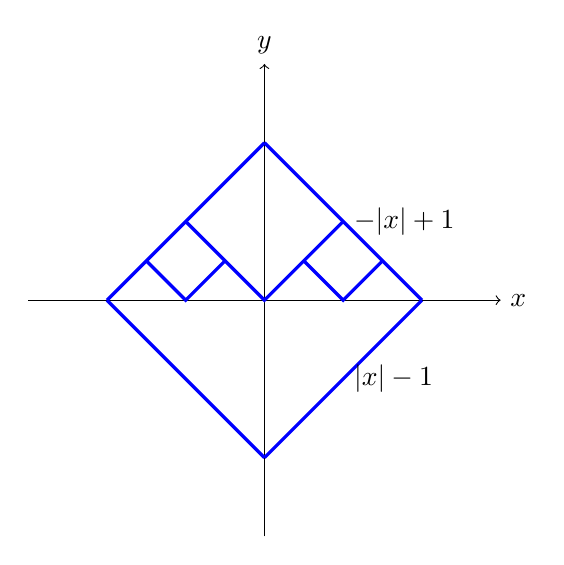
\begin{tikzpicture}[scale=2]

% Axis
      \draw[->] (-1.5,0.0) -- (1.5,0.0) node[anchor=west] {$x$};
      \draw[->] (0.0,-1.5) -- (0.0,1.5) node[anchor=south] {$y$};
% Radmacher Functions
    %k=0
      \begin{scope}[draw=blue,line width=1.2pt]
        \draw (-1.0,0.0) -- (0.0,1.0);
        \draw (0.0,1.0)  -- (0.5,0.5) node[anchor=west] {$-|x|+1$} -- (1.0,0.0);

        \draw (-1.0,0.0)  -- (0.0,-1.0);
        \draw (0.0,-1.0)  -- (0.5,-0.5) node[anchor=west] {$|x|-1$} -- (1.0,0.0);
%k=1
        \draw (-0.5,0.5) -- (-0.0,0.0) -- (0.5,0.5);
%k=2
        \draw (-0.75,0.25) -- (-0.5,0.0) -- (-0.25,0.25);
        \draw (0.25,0.25) -- (0.5,0.0) -- (0.75,0.25);
      \end{scope}

    \end{tikzpicture}
  \end{center}
  \caption{Funzioni di \emph{Readmacher}. Soluzioni quasi ovunque dell'equazione einoidale.}
  \label{fig:cp2-01}
\end{figure}

Nel 1982 Crandal and lions introdussero una differente nozione di soluzione debole (soluzioni viscose \cite[vedi][]{crand:lion}) che si comporta bene per molti PDE del primo e del secondo ordine, soddisfacendo proprietà di esistenza, unicità e stabiltà. 
%%%%%%%%%%%%%%%%%%%%%%%%%%%%%%%%%%%%%%%%%%%%%%%%%%%%%%%%%%%%%%%%%%%%%%%%%%
%
%                            Section 2.2
%
%
%%%%%%%%%%%%%%%%%%%%%%%%%%%%%%%%%%%%%%%%%%%%%%%%%%%%%%%%%%%%%%%%%%%%%%%%%%
\section{Nozione di soluzioni viscose}
Inziamo col introdurre la definizione di soluzione viscosa per PDE del secondo ordine, cioè equazioni del tipo
\begin{equation}
\label{eq:cp2-02}
F(x,u,Du,D^2u) = 0\text{ con }F:\mathbb{R}^N\times\mathbb{R}\times\mathbb{R}^N\times S(N)\to \mathbb{R},
\end{equation}
con $S(N)$ insieme delle matrici simmetriche $N\times N$, $u$ una funzione a volori reali definita in un sottoinsieme $\mathcal{O}$ di $\mathbb{R}^N$ e $Du$,$D^2u$ corrispondono al gradiente ed alla matrice delle derivate seconde di $u$. Al fine di applicare la teoria a un equazione del tipo \eqref{eq:cp2-02} (\cite[vedi][2]{crand:lion}), richiederemo che $F$ soddisfi le seguenti propietà
\begin{gather}
\label{eq:cp2-03}
F(x,r,p,X) \leq F(x,s,p,X) \quad \forall\,r\leq s,\\
\label{eq:cp2-04}
F(x,r,p,X) \leq F(x,r,p,Y) \quad \forall\,Y\leq X,
\end{gather}
con $r,s\in \mathbb{R},X,Y\in S(N)$ and $S(N)$ equipaggiato del solito ordine tra matrici. Se $F$ soddisfa \eqref{eq:cp2-03} allora si dirà \emph{ellitticamente degenere}, mentre se soddisfa \eqref{eq:cp2-04} si dirà \emph{propria}.

Da qui in avanti assumeremo sempre che $F$ soddisfi \eqref{eq:cp2-03} e \eqref{eq:cp2-04} e che sia continua, a meno che non venga detto diversamente. Prima di enunciare la definizione vediamo un po qual è l'idea. Supponiamo che $u\in C^2$ su $\mathbb{R}^n$ e che
\[
F(x,u(x),Du(x),D^2u(x))\leq 0\, \forall x\in\mathbb{R}^n,
\]
cioè $u$ è una sottosoluzione classica di $F=0$. Supponiamo $\phi\in C^2$ e $\hat{x}$ sia un massimo locale per $u-\phi$, dall'analisi  questo implica che $Du(\hat{x})=D\phi(\hat{x})$ e $D^2u(\hat{x})\leq D^2\phi(\hat{x})$, quindi per \eqref{eq:cp2-03},
\[
F(x,u(\hat{x}),D\phi(\hat{x}),D^2\phi(\hat{x}))\leq F(x,u(x),Du(x),D^2u(x))\leq 0.
\]
Gli estremi di questa diseguaglianza non dipendono dalle derivate di $u$, quindi possiamo considerare un arbitraria funzione $u$ essere sotto soluzione di $F=0$ se
\begin{equation}
  \label{eq:cp2-01-add}
  F(x,u(\hat{x}),D\phi(\hat{x}),D^2\phi(\hat{x}))\leq 0
\end{equation}
ogniqualvolta $\phi\in C^2$ e $\hat{x}$ massimo locale di $u-\phi$.
Inoltre  per $x$ vicino a $\hat{x}$ è vero che $u(x)\leq u(\hat{x})-\phi(\hat{x}) + \phi(\hat{x})$, poichè $\phi\in C^2$ usando Taylor otteniamo
\begin{equation}
  \label{eq:cp2-05}
  u(x)\leq u(\hat{x})-\left<p,x-\hat{x}\right> + \frac{1}{2}\left<X(x-\hat{x}),x-\hat{x}\right> + o(|x-\hat{x}|^2)\,\, x\to\hat{x}
\end{equation}
con $p=D\phi(\hat{x})$ e $X=D^2\phi(\hat{x})$. Possiamo osservare che se la \eqref{eq:cp2-05} è soddisfatta per qualche $(p,X)\in\mathbb{R}^n\times S(N)$ e $u$ è due volte differenziabile, allora $p=Du(\hat{x})$ e $D^2u(\hat{x})\leq X$. Quindi se $u$ è una soluzione classica per $F\leq 0$ segue che $F(x,u(x),p,X)\leq 0$ ogni qual volta è vera la \eqref{eq:cp2-05}. Ora possiamo dare la definizione di soluzione viscosa, che si basa proprio sulla \eqref{eq:cp2-05}
\begin{definizione}
\label{def:cp2-01}
Sia $F$ propria ed ellittica degenere e $\mathcal{O}\subset\mathbb{R}^n$.
Una sottosoluzione viscosa di $F=0$ su $\mathcal{O}$ è una funzione $u:\mathcal{O}\to\mathbb{R}$ continua tale che
\begin{equation}
  \label{eq:cp2-06}
  F(x,u(x),p,X)\leq 0\quad\forall x\in\mathcal{O}\text{ and }(p,X)\in J_{\mathcal{O}}^{2,+}u(x).
\end{equation}
Similmente, una sopra soluzione viscosa di $F=0$ su $\mathcal{O}$ è una funzione continua tale che
\begin{equation}
  \label{eq:cp2-07}
  F(x,u(x),p,X)\geq 0\quad\forall x\in\mathcal{O}\text{ and }(p,X)\in J_{\mathcal{O}}^{2,-}u(x).
\end{equation}
Infine, $u$ è una soluzione viscosa se è sia sotto che sopra soluzione.
\end{definizione}
Dove $J_{\mathcal{O}}^{2,+}u(x)$ rappresenta il \emph{superjet} del secondo ordine di $u$ nel puto $x$. Più precisamente sia $\mathcal{O}\subset\mathbb{R}^N$ arbitrario%
\footnote{Nelle dimostrazio di esistenza, unicità e confronto sarà richiesto essere localmente compatto \cite[vedi][10]{crand:lion}}
,  $u:\mathcal{O}\to\mathbb{R}$ e $\hat{x}\in\mathcal{O}$ allora
\[
J_{\mathcal{O}}^{2,+}u(\hat{x}) = \left\{(p,X)\in\mathbb{R}^n\times S(N):\,\text{ vale la \eqref{eq:cp2-05} per }\mathcal{O}\ni x\to\hat{x}\right\},
\]
quindi $J_{\mathcal{O}}^{2,+}u(x)$ definisce una mappa da $\mathcal{O}$ ad un sottoinsieme di $\mathbb{R}^n\times S(N)$. Una definizione simile si ottiene per il \emph{subjet} $J_{\mathcal{O}}^{2,-}u(x)$ basta invertire il segno della disuguaglianza.
\begin{osservazione}
Come si può notare dalla definizione, il ``superjet'' (lo stesso vale per il ``subjets'') dipende dall'insieme $\mathcal{O}$, tuttavia si può notare che il suo valore è lo stesso per tutti quegli insiemi $\mathcal{O}$ per i quali $x$ è un punto interno.  
\end{osservazione}

\begin{osservazione}
Nella definizione di soluzione viscosa, la richiesta di continuità di $u$ può essere sostituita con quella di semicontinuà superiore(\emph{upper semicontinuos}) per le sotto soluzione e semicontinuà inferiore(\emph{lower semicontinuos}) per le sopra soluzione. Inoltre, notare che una funzione semicontinua sia superiormente che inferiormente è continua. Ricordiamo che  $u:\mathcal{O}\to\mathbb{R}$ è
\begin{enumerate}
  \item \emph{upper semicontinuos} in $\hat{x}\in\mathcal{O}$ se:
    \[
      \limsup_{x\to\hat{x}}u(x)\leq u(\hat{x}).
    \]
  \item \emph{lower semicontinuos} in $\hat{x}\in\mathcal{O}$ se:
    \[
      \liminf_{x\to\hat{x}}u(x)\geq u(\hat{x}).
    \]
\end{enumerate}  

Seguendo la discussione fatta ad inizio sezione, se $u$ è una soluzione viscosa di $F\leq 0$, $\phi\in C^2$ in un intorno di $\mathcal{O}$ e $u-\phi$ ha un massimo locale in $\hat{x}\in\mathcal{O}$, allora è vera la \eqref{eq:cp2-01-add} ( stesso ragionamento per le sopra soluzioni). Questo motiva la richiesta per $u$ di essere semicontinua dall'alto (rispettivamente dal basso per le sopra soluzioni), in quanto è facile produrre massimi per funzioni semicontinue dall'alto.
Possiamo dire di più, la validità di \eqref{eq:cp2-01-add} per tutte le $\phi\in C^2$ tale che $u-\phi$ ha un massimo locale relativo ad $\mathcal{O}$, con $u$ semicontinua dall'alto, equivale a dire che $u$ è una sotto soluzione viscosa.  Infatti si può mostrare che se $\hat{x}\in\mathcal{O}$ allora
\[
J_{\mathcal{O}}^{2,+}u(\hat{x}) = \left\{(D\phi(\hat{x}),D^2\phi(\hat{x})):\,\phi\in C^2\text{ e $u-\phi$ ha massimo locale in $\hat{x}$}\right\},
\]

\end{osservazione}

\begin{osservazione}
Si può facilmente verificare che se $u\in C^2$ è soluzione classica di \eqref{eq:cp2-02} ed $F$ è elliticamente degenere, allora $u$ è soluzione viscosa.
\end{osservazione}

\begin{esempio}
Riprendiamo l'equazione eiconale \eqref{eq:cp2-01} e mostriamo che la funzione $u(x) = -|x| + 1$ è una soluzione viscosa. Partiamo dall'osservare che questa funzione risolve classicamente l'equazione in $\mathbb{R}\setminus\{0\}$, quindi
calcoliamoci rapidamente il ``superjets'' e il ``subjets'' in $\hat{x}=0$
\[
\begin{aligned}
  J^{2,+}u(0) &= \left\{\left((-1,1)\times\mathbb{R}\right)\cup\left(\{-1,1\}\times [0,+\infty)\right)\right\}, \\
  J^{2,-}u(0) &= \left\{\emptyset\right\},
\end{aligned}
\]
applicando la definizione \ref{def:cp2-01} si osserva che $|p|\leq 1$ è vera per ogni $(p,X)\in J^{2,+}u(0)$, quindi è sotto soluzione e che $|p|\geq 1$ è banalmente verificata in quanto $J^{2,-}u(0)=\emptyset$. In conclusione $u(x)=-|x|+1$ e soluzione viscosa di \eqref{eq:cp2-01}.  
\end{esempio}

La definizione di soluzione viscosa qui presentata, può essere estesa anche al caso di equazioni paraboliche cioè del tipo
\begin{equation}
\label{eq:cp2-08}
u_t + F(t,x,u,Du,D^2u) = 0,
\end{equation}
dove ora $u=u(t,x)$ e $Du$, $D^2u$ stanno per $D_xu$ e $D^2_xu$. Per farlo dobbiamo ridefinire gli insiemi $J_{\mathcal{O}}^{2,\pm}$. Sia $\mathcal{O}\subset\mathbb{R}^N$, $T>0$ e $\mathcal{O}_T = (0,T)\times\mathcal{O}$, denotiamo con $\mathcal{P}_{\mathcal{O}}^{2,\pm}$ la variante parbolita dei ``superjets'' e ``subjets'' e andiamoli a definire; se $u:\mathcal{O}\to\mathbb{R}$ allora $\mathcal{P}_{\mathcal{O}}^{2,+}u(s,z)$ è costituito da $(a,p,X)\in\mathbb{R}\times\mathbb{R}^N\times S(N)$ se $(s,z)\in\mathcal{O}_T$ e
\[
\begin{aligned}
  u(t,x)\leq &u(s,z) +a(t-s)+\left<p,x-z\right>+\frac{1}{2}\left<X(x-z),x-z\right> \\
  &+o(|t-s|+|x-z|^2)\text{ per }\mathcal{O}_T\ni (t,x)\to(s,z),
\end{aligned}
\]
similarmente possiamo definire $\mathcal{P}_{\mathcal{O}}^{2,-}u(s,z)=-\mathcal{P}_{\mathcal{O}}^{2,+}(-u(s,z))$. Quindi in conclusione una sotto soluzione di \eqref{eq:cp2-08} su $\mathcal{O}_T$ è una funzione $u$ semicontinua dall'alto tale che
\[
a+F(t,x,u(t,x),p,X)\leq 0\text{ per }(t,x)\in\mathcal{O}_T,(a,p,X)\in\mathcal{P}_{\mathcal{O}}^{2,+}u(t,x),
\]
e una sopra soluzione una funzione semicontinua dal basso tale che
\[
a+F(t,x,u(t,x),p,X)\geq 0\text{ per }(t,x)\in\mathcal{O}_T,(a,p,X)\in\mathcal{P}_{\mathcal{O}}^{2,-}u(t,x),
\]
e quindi un soluzione viscosa se sono verificate entrambe le diseguaglianze.
Le definizioni si posso estendere anche nel caso in cui ci siano delle discontinutà sia per $u$ che per $F$, prima di procedere richiamiamo la definizione di inviluppo semicontinuo.

Per risultati di esistenza, unicità e confronto sia per equazioni del tipo \eqref{eq:cp2-02} che \eqref{eq:cp2-08} \cite[vedi][]{crand:lion,giga:main}.
